% ================================================
% setting
% ================================================

% upLaTeXの環境でコンパイルの場合は"u"がつく
% \documentclass[uplatex, 12pt, a4j, fleqn]{ujreport}
\documentclass[uplatex, 12pt, a4j, fleqn]{ujbook}

% begin.texに使用するパッケージなどの記述

% 読み込ませたいパッケージを記述する

% 太字が使える
\usepackage{bm}
%\usepackage{AIthesis}
% 図の関係で必要
\usepackage[dvipdfmx]{graphicx}

% pdf読み込みできるやつ
%\usepackage{mediabb}

% 数式のやつ
\usepackage{amsmath,amssymb}
\usepackage{amsthm}
\usepackage{longtable}
\usepackage{enumerate}
\usepackage{float}
\usepackage{wrapfig}
\usepackage{ascmac}
% 表に斜線を引ける、styファイルは要ダウンロード
%http://www.biwako.shiga-u.ac.jp/sensei/kumazawa/tex/slashbox.html
%\usepackage{slashbox}
% URLを直接記述できる、\url{}
\usepackage{url}
\usepackage{multirow}
\usepackage{ccaption}
\usepackage{afterpage}
\usepackage[a4paper]{geometry}
% 参考文献を本文で引用するときに使うやつ
\usepackage{cite}
% 図を横にならべて(a) OOとかできるやつ
\usepackage{subcaption}
% \usepackage[subrefformat=parens]{subcaption}
% まとめてコメントアウトできるやつ
\usepackage{comment}
% 表のセル内で自動改行するために必要
\usepackage{tabularx}
% 図の配置で[h]を指定した時に、確実にその位置に配置するやつ
\usepackage{here}
% \newpageで改ページ(文章変だけど)
\usepackage{afterpage}

% 図の配置を変えるやつ
%\usepackage[colorlinks=false,urlcolor=blue]{hyperref}




% 行数設定など行う
\makeatletter
\def\mojiparline#1{
    \newcounter{mpl}
    \setcounter{mpl}{#1}
    \@tempdima=\linewidth
    \advance\@tempdima by-\value{mpl}zw
    \addtocounter{mpl}{-1}
    \divide\@tempdima by \value{mpl}
    \advance\kanjiskip by\@tempdima
    \advance\parindent by\@tempdima
}
\makeatother
\def\linesparpage#1{
    \baselineskip=\textheight
    \divide\baselineskip by #1
}

% 余白の設定
% A4(297mm)
\setlength{\textheight}{227truemm}
\setlength{\headheight}{20truemm}
\setlength{\topskip}{20truemm}
\setlength{\headsep}{15truemm}
\setlength{\footskip}{0truemm}
\addtolength{\topmargin}{-1truein}

% セクションの番号付けの深さを設定
% 例えば3を指定すると、\subsubsubsectionまでは番号がつく
\setcounter{secnumdepth}{5}

% 図の保存場所
\graphicspath{{../fig/}}

% ================================================
% Document (start)
% ================================================

% ドキュメントの開始
\begin{document}

% 一行あたり文字数の指定
\mojiparline{35}
% 1ページあたり行数の指定
\linesparpage{27}


% タイトルの出力
% title.texを読み込んでる書いておく

% 表紙

\begin{titlepage}
	\begin{center}
		\vspace*{30truept}
		{\Large 令和○○年度 修士論文} \\
		\vspace{100truept}
		{\LARGE TeXの}\\
		\vspace{12truept}
		{\LARGE テンプレート} \\
		\vspace{80truept}
		{\large
		xx大学\\
		xx専攻 xx研究室\\
		指導教員 xx 教授\\
		}
		\vspace{50truept}
		{\large 学籍番号 xxxxxx}\\ % 学籍番号
	
		\vspace{10truept}
		{\large  oo oo}\\ % 著者
	
		\vspace{50truept}
		{\large 令和○○年○月○日 提出}\\ % 提出日
	\end{center}
\end{titlepage}




% 図番号の後を":"をスペースに置き換える
% お好みで設定
\captionsetup{labelsep=space}
\renewcommand{\include}[1]{}
\renewcommand\documentclass[2][]{}

% 目次用にページ番号の付け方を"roman"に変えておく
\pagenumbering{roman}
% 目次の出力
\tableofcontents
% 図目次の表示
\listoffigures
% 表目次の表示
\listoftables

% 各チャプター分けしたファイルを読み込む

% ====================================
% chapter 1
% ====================================

\chapter{TeXのテンプレートを作ってみました}

% ページ番号をリセット
\setcounter{page}{1}
% ページ番号の付け方をromanからarabicに変えておく
\pagenumbering{arabic}


\section{はじめに}
TeXのテンプレートを作ってみました.
まずはじめ,作成者の使用上コマンドは\verb|¥|ではなく\verb|\|にしています.
理由はMac導入時のデフォルトであったこととかっこいいからです.
お手数ですが,最初にメモ帳などなんでもいいので各ファイルの\verb|\|を\verb|¥|に置換してください.
気が向いたら\verb|¥|バージョンも作ります.

コンパイル環境はなんでもいいですが,latexmkというものを使うと便利です.
普通TeXはラベルをひも付けたりなどの関係で複数回コンパイルが必要になりますが,それらを一括でやってくれます.
本記事ではlatexmkを使ったコンパイル環境を構築します.

あと,ささやかな注意事項ですが,ファイル名は半角文字のみ使用をお願いします.

\section{TeXのインストールと設定}

Macの場合はMacTeXを入れるだけでok.
WinやLinuxの人はTeX Liveを入れれば間違いないみたいです.

latexmkは".latexmkrc"という設定ファイルを作る必要があります.
頭にドットがついているのに注意してください.
作成先はHomeディレクトリか,作業ディレクトリに作れば大丈夫ですが,作業用のディレクトリがおすすめです.
このサンプルでは既に作成済ですが,簡単に中身に触れておきます.

今回は".latexmk"に以下を書き込んでいます(正確には若干違いますが、直すのが面倒).

\begin{verbatim}
#!/usr/bin/env perl
$latex            = 'uplatex -synctex=1 -halt-on-error';
$latex_silent     = 'uplatex -synctex=1 -halt-on-error -interaction=batchmode';
$bibtex           = 'upbibtex';
$biber            = 'biber --bblencoding=utf8 -u -U --output_safechars';
$dvipdf           = 'dvipdfmx %O -o %D %S';
$makeindex        = 'mendex %O -o %D %S';
$max_repeat       = 5;
$pdf_mode         = 3;
\end{verbatim}

ここで注意なのが,タイプセットの環境がuplatexとplatexの人がいます.
ここではuplatexを使っていますが,もしplatexを使う場合は以下のように書き換えてください.

\begin{verbatim}
#!/usr/bin/env perl
$latex            = 'platex -synctex=1 -halt-on-error';
$latex_silent     = 'platex -synctex=1 -halt-on-error -interaction=batchmode';
$bibtex           = 'pbibtex';
$biber            = 'biber --bblencoding=utf8 -u -U --output_safechars';
$dvipdf           = 'dvipdfmx %O -o %D %S';
$makeindex        = 'mendex %O -o %D %S';
$max_repeat       = 5;
$pdf_mode         = 3;
\end{verbatim}
各設定の意味や他の設定については各自で検索していただければと思います.

設定を書き込んだら,ターミナル上でTeXのソースファイルのある作業ディレクトリまで移動し,次のコマンドを打つとPDFが作成されます.
\begin{verbatim}
latexmk main.tex
\end{verbatim}
main.texは各自のソースファイル名へ適宜読み替えてください.
上記コマンドを毎回呼び出すのは面倒なので,ファイルが変更されるたびにコンパイルできるよう引数を与えます.
\begin{verbatim}
latexmk -pvc main.tex
\end{verbatim}
これで幸せなTeXコンパイル環境の出来上がりです.

コンパイルするとたくさんの中間ファイルたちが生成されて見た目や管理上邪魔になります.
ここで朗報です.
Bashなどが利用できるMacやLinux環境のみなさんには朗報なんです.
本サンプルの直下に"shell"というフォルダが見えますでしょうか.
"shell"内には3つの.shの拡張子でファイルがあり,それぞれ以下のような効果を発揮してしまうのです.
スーパー執筆モードになっているときはchange2build\_loopd\_and\_rm\_files.shを裏で実行しておくと便利です.
\begin{description}
    \item[rm\_files.sh]\mbox{}\\
        生成された中間ファイルの削除
    \item[build\_and\_rm\_files.sh]\mbox{}\\
        一回だけコンパイルしてrm\_files.shを実行
    \item[change2build\_loopd\_and\_rm\_files.sh]\mbox{}\\
        変更を監視して自動コンパイルし,終了時にrm\_files.shを実行
\end{description}
なお,Winは知りません.

\section{TeXのエディタ}

TeXは拡張子こそ.texになっていますが,実際に編集を行うのは文章が書けるソフトであればなんでもいいです.
極端な話し,メモ帳などでも大丈夫です.
しかし,編集するに当たって補完機能やコマンドのハイライトなどしてくれると作業効率も上がりますので,TeXShopやTeXWorks,拡張機能をインストールできるエディタ(AtomやVSCode)などの利用をお勧めします.
最強のエディタはVimと信じて疑っていない私ですが,作業効率重視でいきましょう.

ちなみにlatexmkではプレビュー用のソフトの設定も書き込めるので適宜Webで調べてみてください.




% ====================================
% chapter 2
% ====================================

\chapter{TeXでよく使うコマンド}

\section{セクション}

\verb|\section|をつけるとセクションわけができる.小分けにしたいときに便利.
\subsection{subsection}
さらに,\verb|\subsection|みたいに、さらなる小分けもできます.\verb|\subsubsection|みたいにsubをつけるほど細かくできます.

\subsection{サブセクションのテスト}

階層が深くなります.

\subsubsection{subsubsection}

めっちゃ階層が深くなります.
subをつけまくるとわかりにくくもなるのであまり階層を深くしすぎないように注意しましょう.

\section{図}

図は別フォルダにまとめておくと便利ですので,本テンプレートではFigというフォルダを作ってその中に図を入れています.

図は次のように出力します.
タイトル名やオプションなどは必要なように書き換えてください(詳しくはWebで!).
\begin{verbatim}
\begin{figure}[指定位置]
    \centering
    \includegraphics[オプション]{ファイル名}
    \caption{タイトル名} %タイトルをつける
    \label{ラベル} %ラベルをつけ図の参照を可能にする
\end{figure}
\end{verbatim}


修論のように大型の論文の場合は,Figフォルダの中で,更にフォルダを小分けしておくと便利です.
ここで,涅槃像を見にいった時に見つけた地蔵の画像を「Fig/ch2/地蔵.jpg」に入れてあるので,出力してみたいと思います(図\ref{fig_地蔵}).
画像が大きいのでオプション"scale"でサイズ調整してます.
ちなみに\verb|\ref{}|を使い{}内にラベル名を書くと番号を引用できます.

\begin{verbatim}
\begin{figure}[]
    \centering
    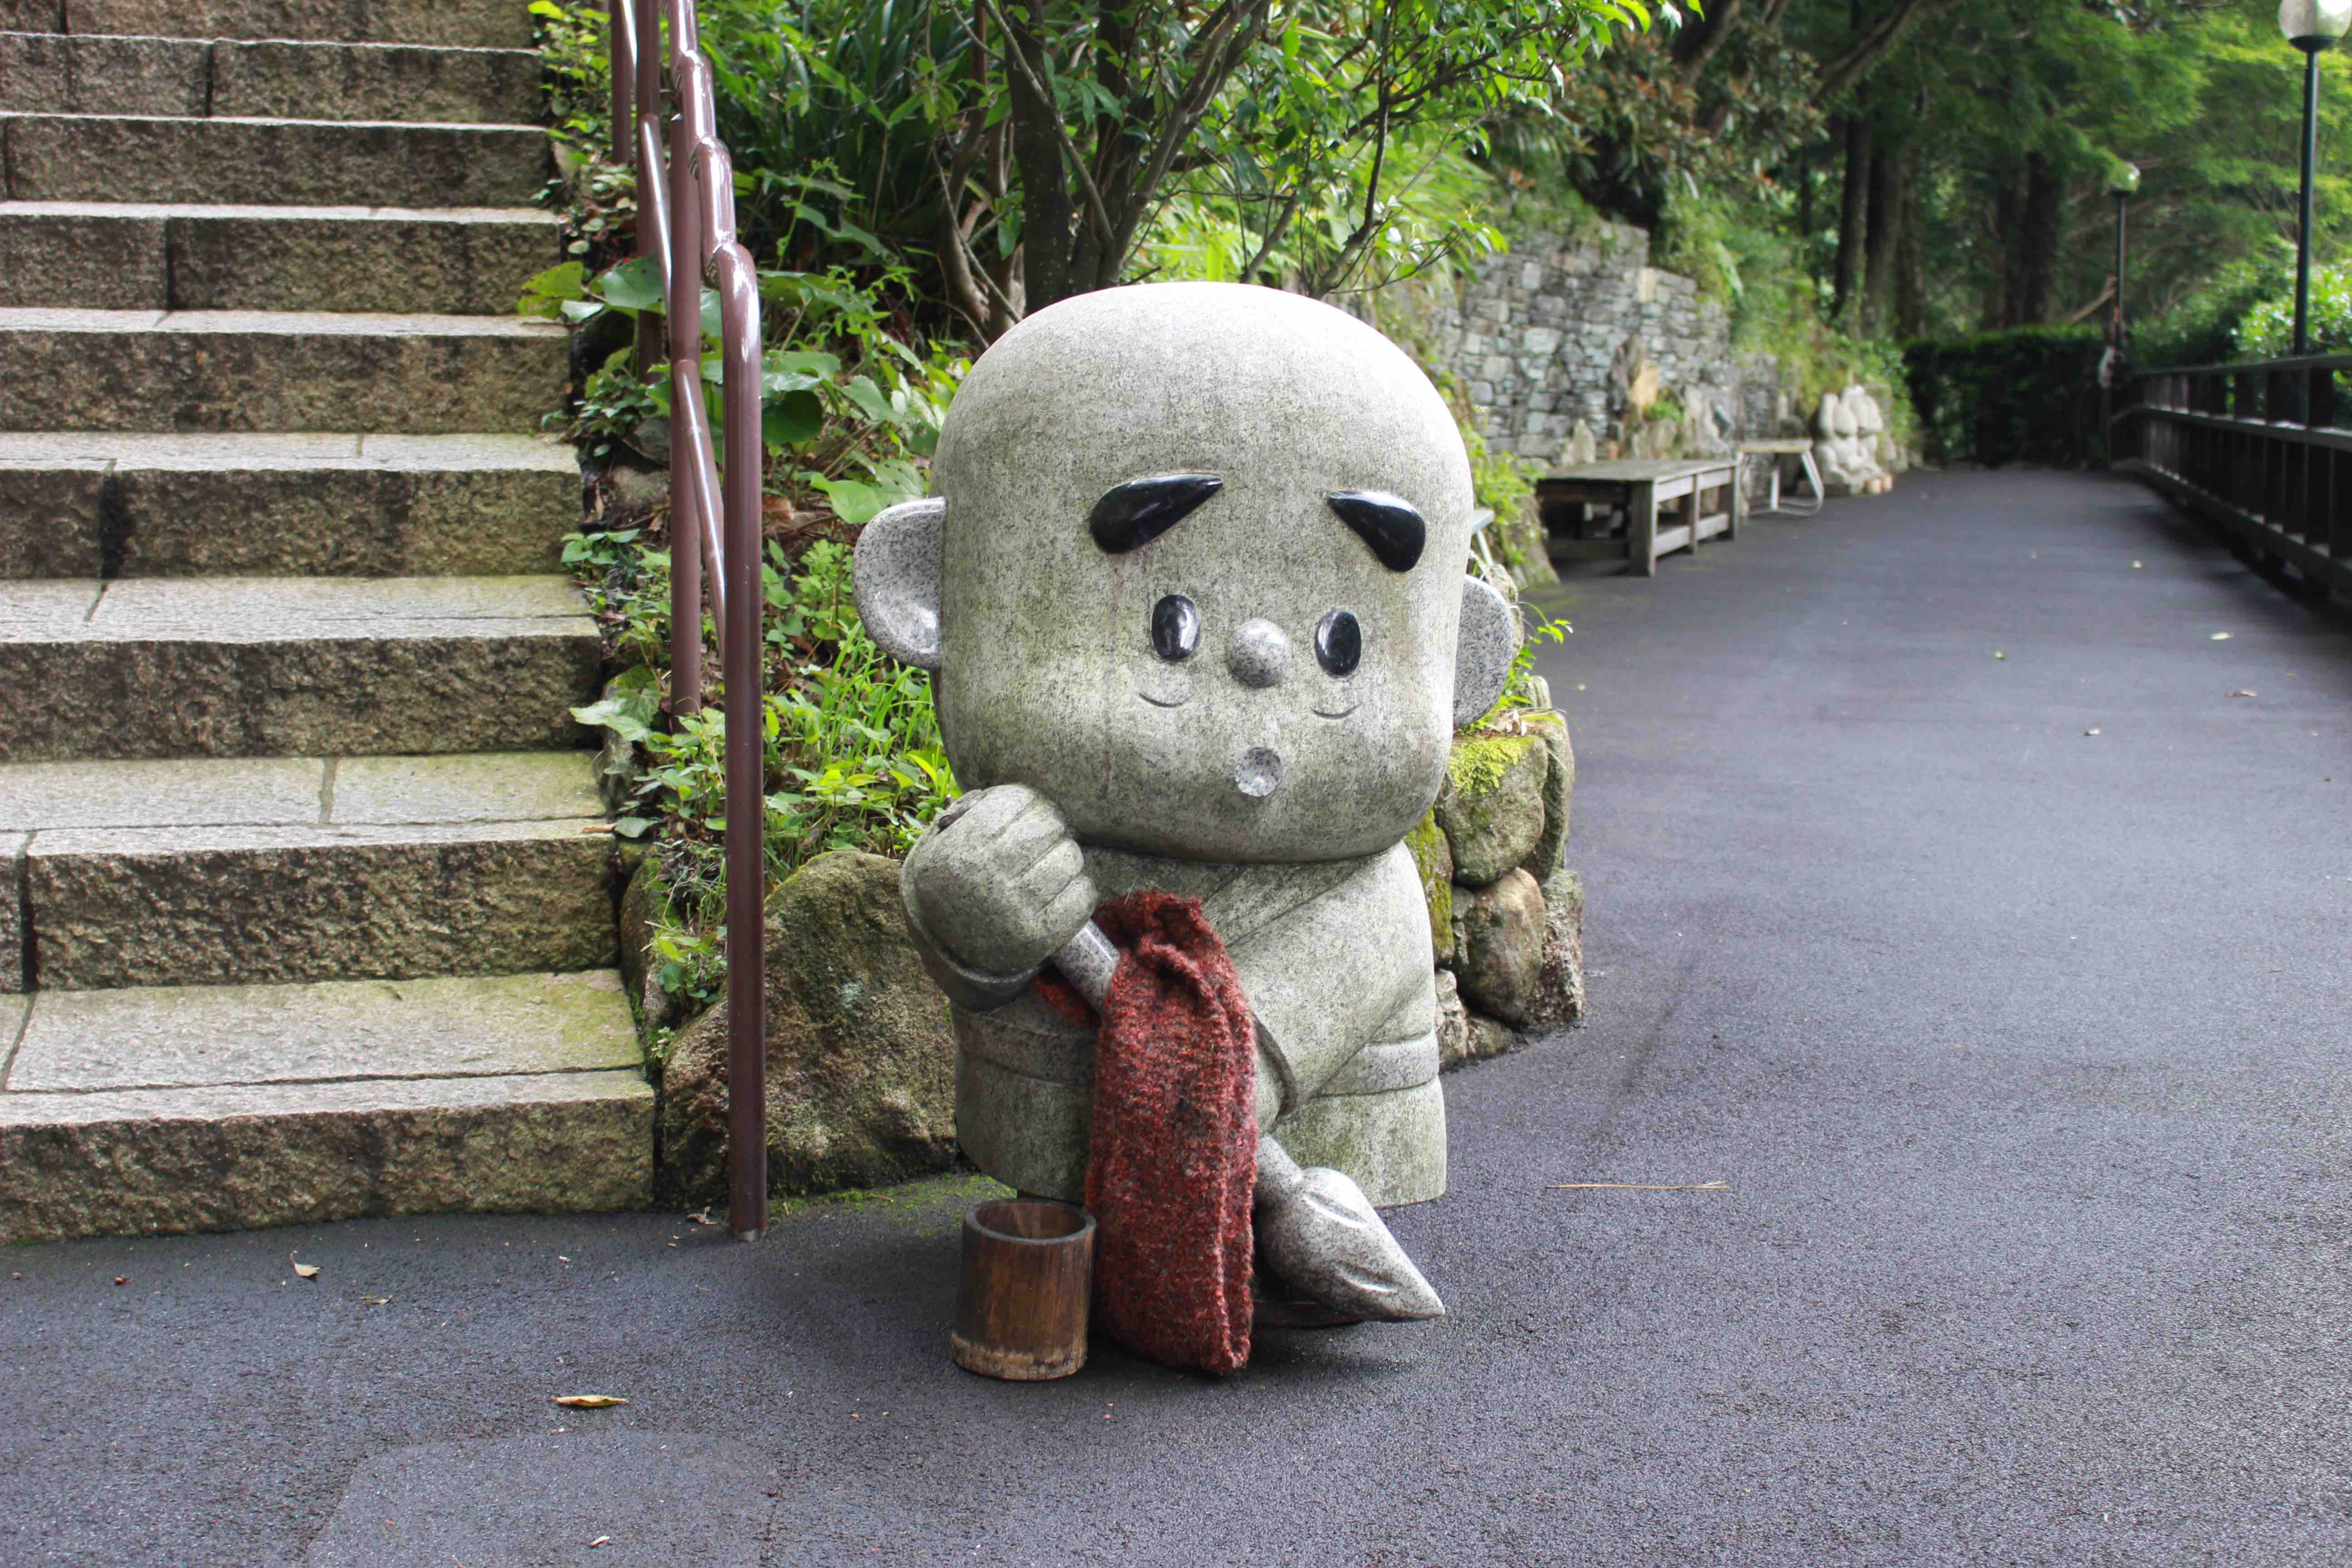
\includegraphics[scale = 0.05]{chapter2/yoshimoto.jpg}
    \caption{涅槃像見にいった時に見つけた地蔵} %タイトルをつける
    \label{fig_地蔵} %ラベルをつけ図の参照を可能にする
\end{figure}
\end{verbatim}

\begin{figure}[]
  \begin{center}
    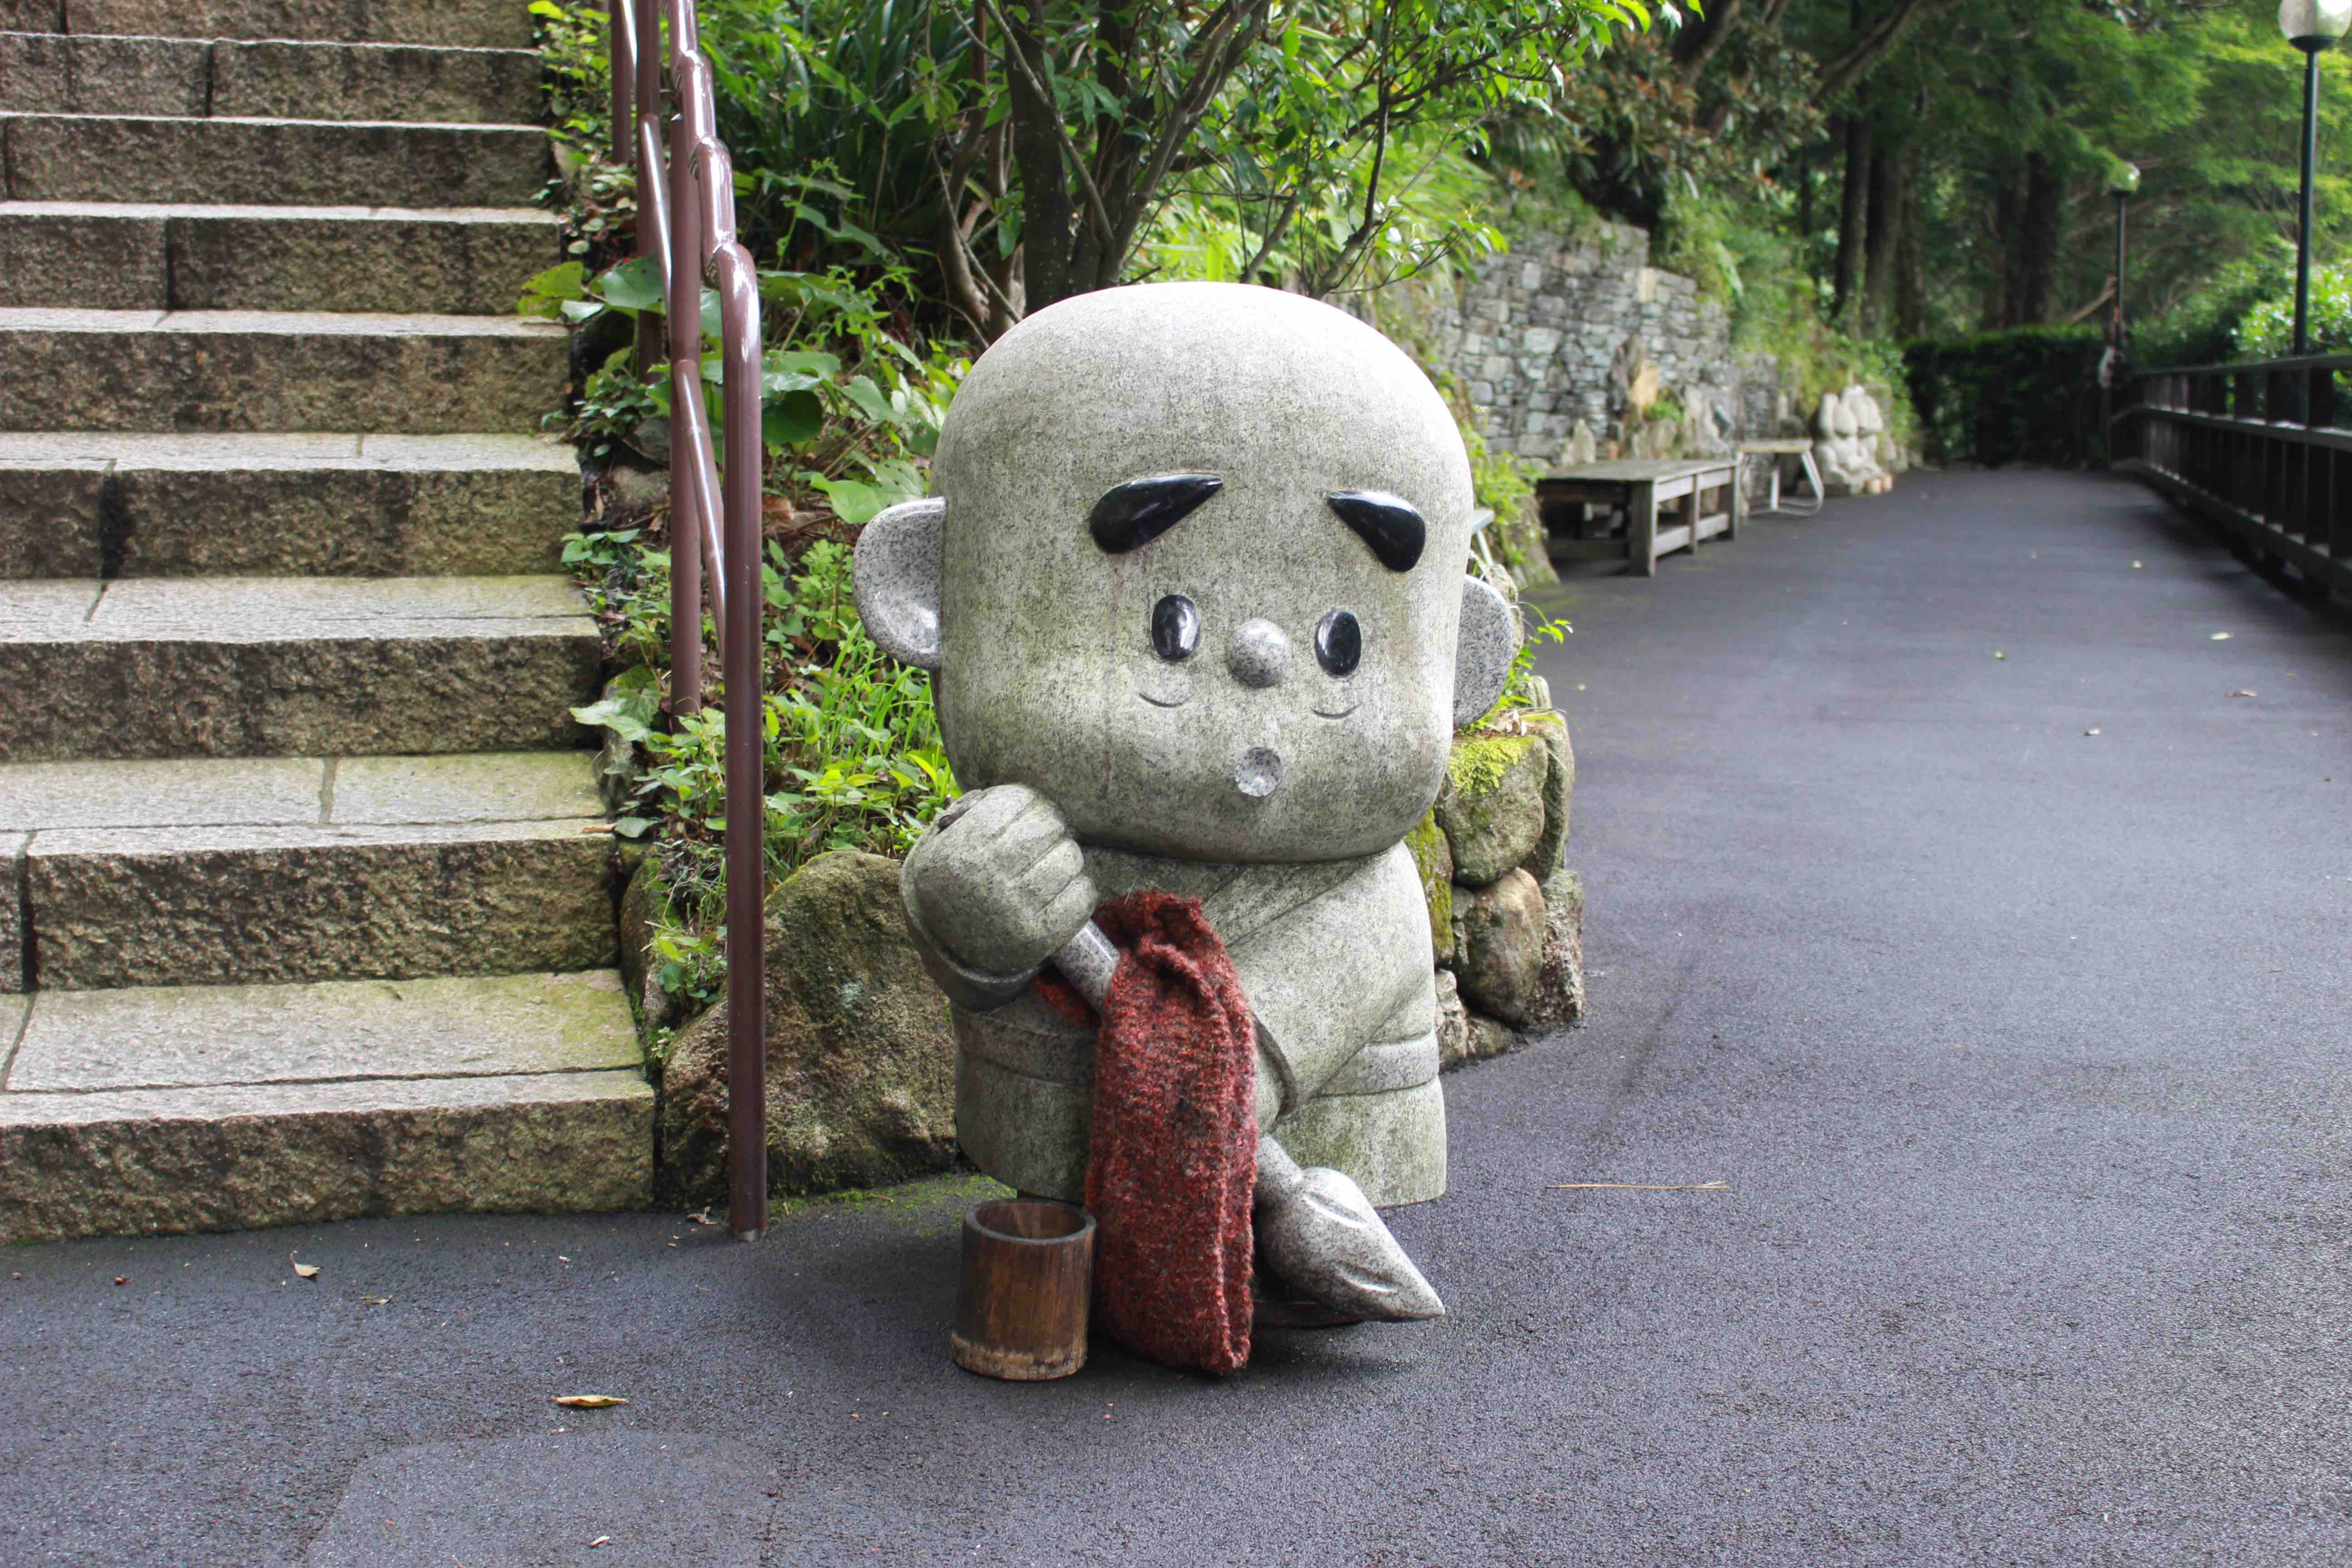
\includegraphics[scale = 0.05]{./chapter2/yoshimoto.jpg}
    \caption{涅槃像見にいった時に見つけた地蔵}
    \label{fig_地蔵}
  \end{center}
\end{figure}

\section{表}
表は結構説明が面倒なので詳細は省きます.
基本的には以下のコマンドで表が出力できます.
TeXで表を書くのは結構面倒です.
\begin{verbatim}
\begin{table}[位置指定]
  \begin{tabular}{列指定}
    表本体・・・
  \end{tabular}
\end{table}
\end{verbatim}

表本体の項目は「\verb|&|」を使って分けます.
また,数式などでも共通ですが,「\verb|\\|」を使って行を変えます.
ここでは簡単に以下の表を出力します.
\begin{verbatim}
\begin{table}[htbp]
  \centering
  \caption{Add caption}
    \begin{tabular}{l|l}
    \multicolumn{2}{c}{master unko} \\ \hline
    unko & unko2 \\
    test & test2 \\
    \end{tabular}
  \label{tab_addlabel}
\end{table}
\end{verbatim}

\begin{table}[htbp]
  \centering
  \caption{適当な表}
    \begin{tabular}{l|l}
    \multicolumn{2}{c}{master unko} \\ \hline
    unko & unko2 \\
    test & test2 \\
    \end{tabular}
  \label{tab_addlabel}
\end{table}

\section{箇条書き}

時には箇条書きをすると見やすくなることがあります.
そんな時は以下のようにするのです.

\begin{verbatim}
\begin{itemize}
    \item unko
    \item test
\end{itemize}
\end{verbatim}

出力結果は以下のようになります.
\begin{itemize}
    \item unko
    \item test
\end{itemize}

\section{参考文献}

参考文献はbibTeXを使うと大変便利です.
みんな積極的に使っていこう.
本テンプレートではref.bibという名前のファイルを作って,その中に記述してます.
詳細はWebを見ていただけたらと思います.
bibTeXはファイル内で実際に使っていない参考文献が書いてあっても,順番がめちゃくちゃであっても,TeXをコンパイルすれば順番通りかつ必要な文献だけ記載してくれます.

参考文献の実際の引用は\verb|\cite{}|を使います.{}の中にはラベルを書きます.
本テンプレートでは適当にref.bibに書き込んである参考文献のラベルを「\verb|ref_tex|」としているので,\verb|\cite{ref_tex}|と書きます.
\begin{itemize}
    \item 例)先行研究としてこんなのが提案されてる\cite{ref_tex}.
\end{itemize}
もし複数の参考文献を参照したい場合は\verb|\cite{label_1,label_2,...}|のようにラベルを「,」で区切ります.

ちなみに論文は有料でPDFがDLできないけどbibTeXならDLできたりします.
その中身をref.texにコピーして形を整えてあげると良いです.


% bibtex 
% {}内を{junsrt}にしないと引用順番にならないので注意
\bibliographystyle{junsrt}
% 関連図書 → 参考文献に変更する
% jbook.clsのthebibliographyは、関連図書と出力するので、
% 		\renewcommand{\bibname}{参考文献}
%  をプレアンブルに入れることで、"参考文献"と変わります。jarticleの場合は、
 % 		\renewcommand{\refname}{参考}

\renewcommand{\bibname}{参考文献}
\bibliography{./etc/ref}
% 以下のように複数ある場合は複数指定できる
% \bibliography{./etc/ref,./etc/ref_2}

% 謝辞

\chapter*{謝辞}
とにかく感謝の気持ちを書こう!!

% ================================================
% Document (end)
% ================================================

\end{document}

